The antimony microelectrode fabrication process is based on the original work of Bard \cite{horrocks1993scanning}.
To create such electrodes, antimony powder (Szka\-ra\-be\-usz, Pécs, Hungary) was melted in a ceramic crucible over a Bunsen burner. Then the molten antimony was pulled into a thick walled borosilicate glass tube ($d_i$=2 mm, $d_o$=10 mm) by applying vacuum using an aspirator on the back opening of the tube.
In this way, a continuous column of solid antimony was sealed into the glass tube.
Then, the glass tube with the antomony inside was melted again.
Since the melting points of antimony and the softening point of the borosilicate glass are very similar, they could be pulled together with standard glass blowing techniques.
After the glass became soft, an antimony containing portion of it was suddenly pulled using tweezers.
With this method, very fine, glass-sealed antimony microwires could be obtained.
After this step, the diameter of the antimony wires was typically around $30~\upmu$m.
If it was necessary, the microwires were pulled even further with a vertical puller (Sutter Instrument, 1 Digital Dr, Novato, CA 94949).
After the pulling stage, the wires were broken into pieces with a length of $3-4$ centimeters.
Then, they were investigated under an optical microscope to select pieces with a continuous antimony wire inside.
Due to the fragile nature of these microelectrodes, they often broke, and several of them were used through the course of my work.
The diameter of the antimony microelectrode used in a particular experiment is always specified in the discussion of that experiment.
To make electrical contact between the measuring instruments and the antimony microwires, a thin copper wire was glued to the glass shielding of antimony wire with conductive silver-epoxy (Amepox Microelectronics, Ltd.
90-268 Lodz Jaracza, Poland), making sure that the epoxy also covered the exposed antimony wire.
After curing the conductive glue for 1 hour at a temperature of 200 $\celsius$, the antimony microelectrodes were ready.
Then the whole assembly was inserted into an empty glass capillary ($d_i=1~$mm).
The remaining space in the capillary was filled with regular epoxy.
This last step increased the mechanical stability of the microelectrode.
All electrodes were tested before usage by calibration in three buffer solutions (pH = 4, 7, 10). 

\paragraph{Antimony pH-sensitive combined macroelectrode}

Home-made antimony/silver combined macroelectrodes were used to study the effect of stirring on the delay in potentiometric measurements with antimony electrodes in general.
To make these electrodes, copper wires were soldered to one end of a $\sim 5~$mm long silver and antimony wires ($d = 1~$mm).
Antimony wires with such diameter were made by pulling molten antimony into a $d_i = 1~$mm glass capillary, the same way that is described in the previous section.
Then, the glass was broken to aquire the antimony wire, which was then trimmed to $\sim 5~$mm length.

Both solder joints were strengthened mechanically by small segments of heatshrink tubes.
The obtained electrodes were carefully pushed down into a glass tube ($d_o = 5~$mm, $d_i=4~$mm) until they both reached the end of the glass tube.
Then, the remaining space in the tube was filled with non-conductive epoxy resin.
Finally, after the resin was cured, the end plate was sanded down to 4000 grit, and polished on three different fiber cloths (Buehler), containing alumina slurry with decreasing particle size; 1$~\upmu$m, 0.3$~\upmu$m and finally 0.05$~\upmu$m. The endresult is depicted in Fig.$~$\ref{fig:sb_macro}.

\begin{figure}
\centering
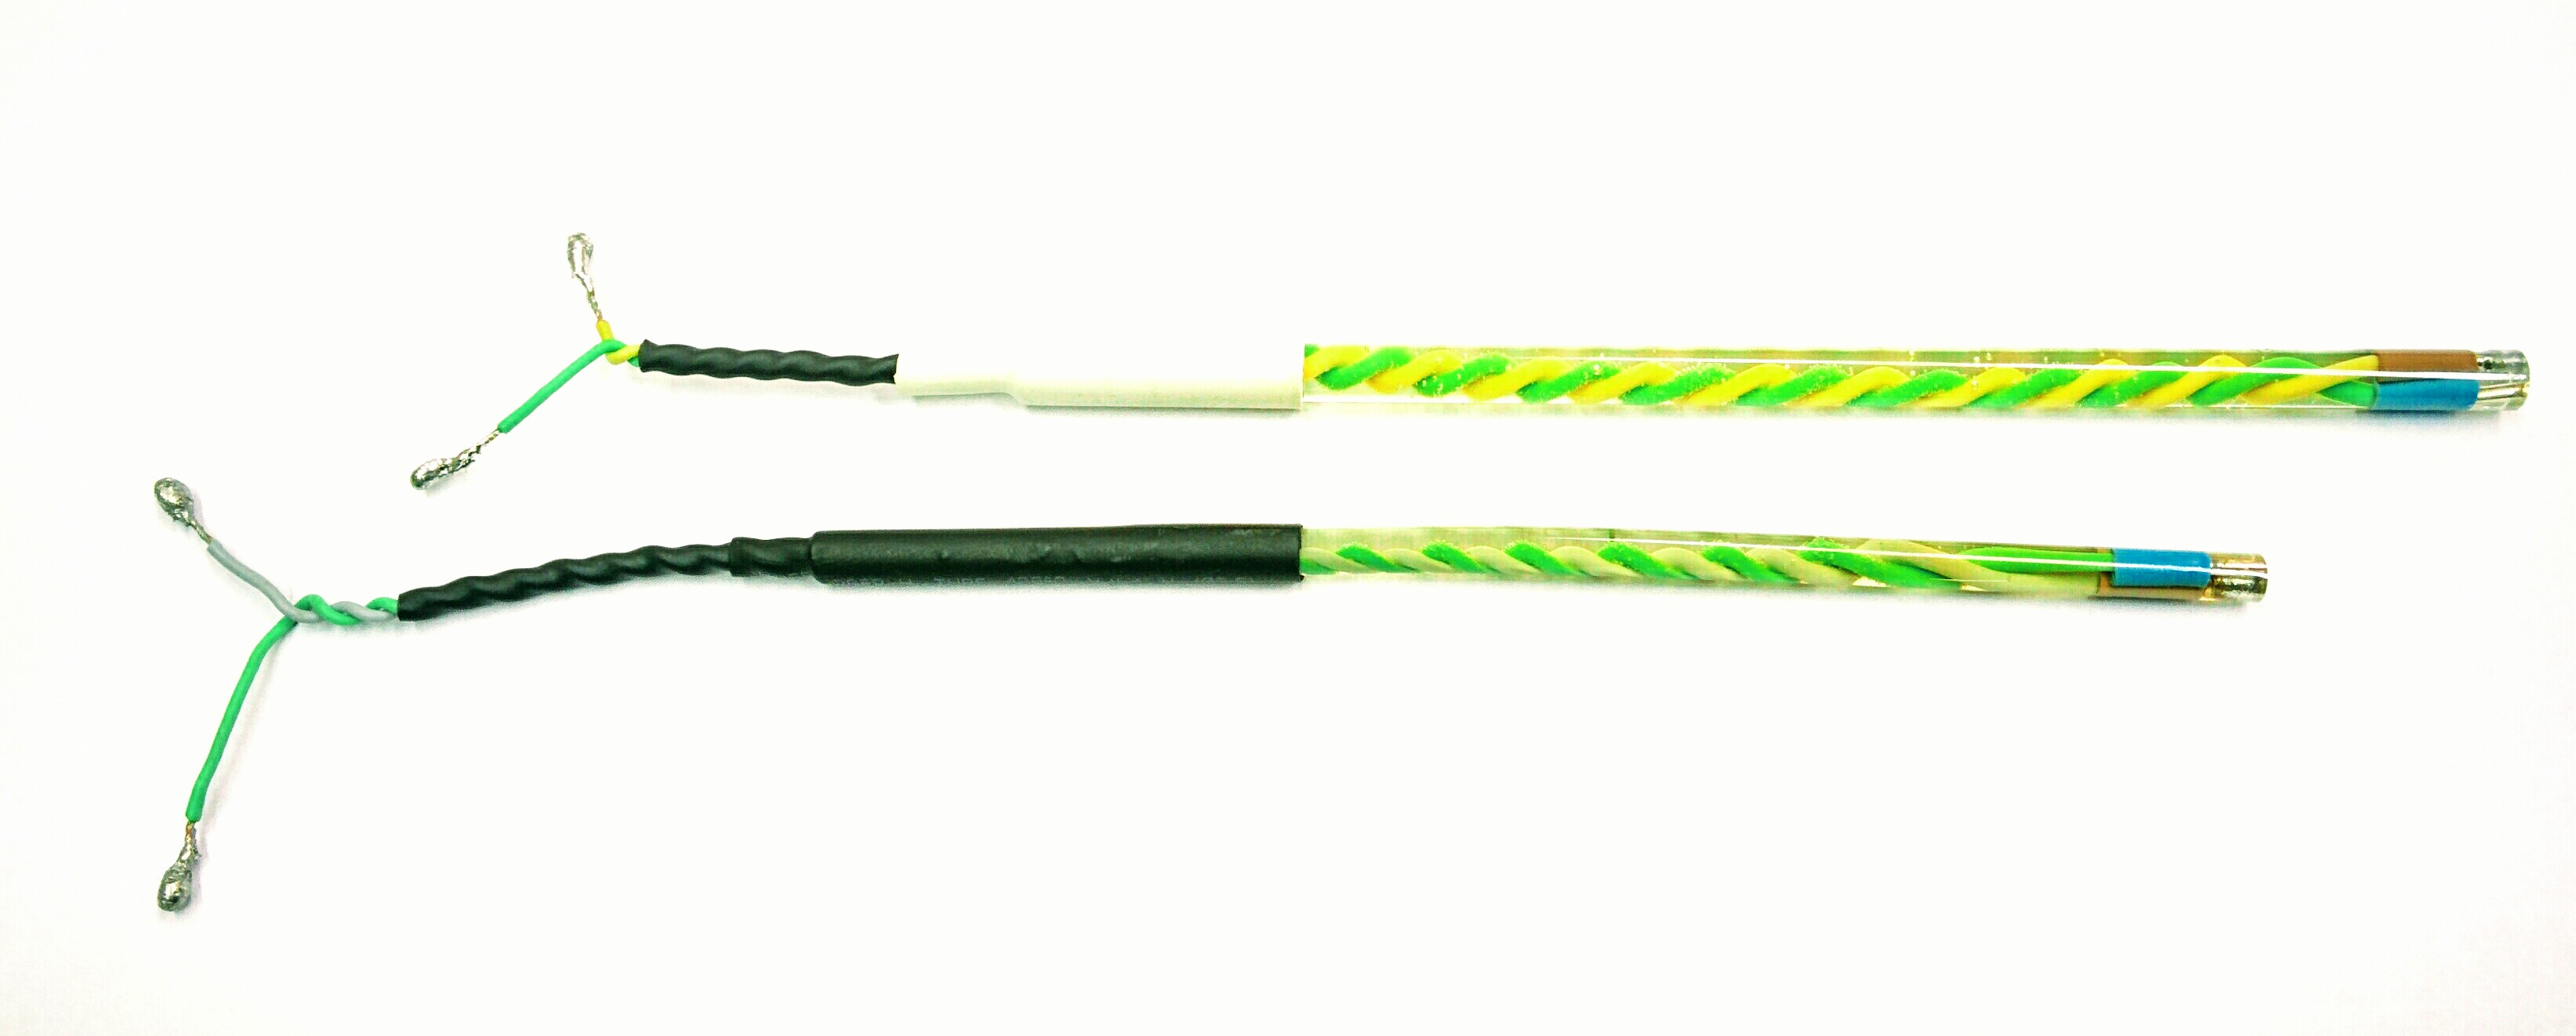
\includegraphics[width=0.693\textwidth]{img/sb_ag_top.jpg}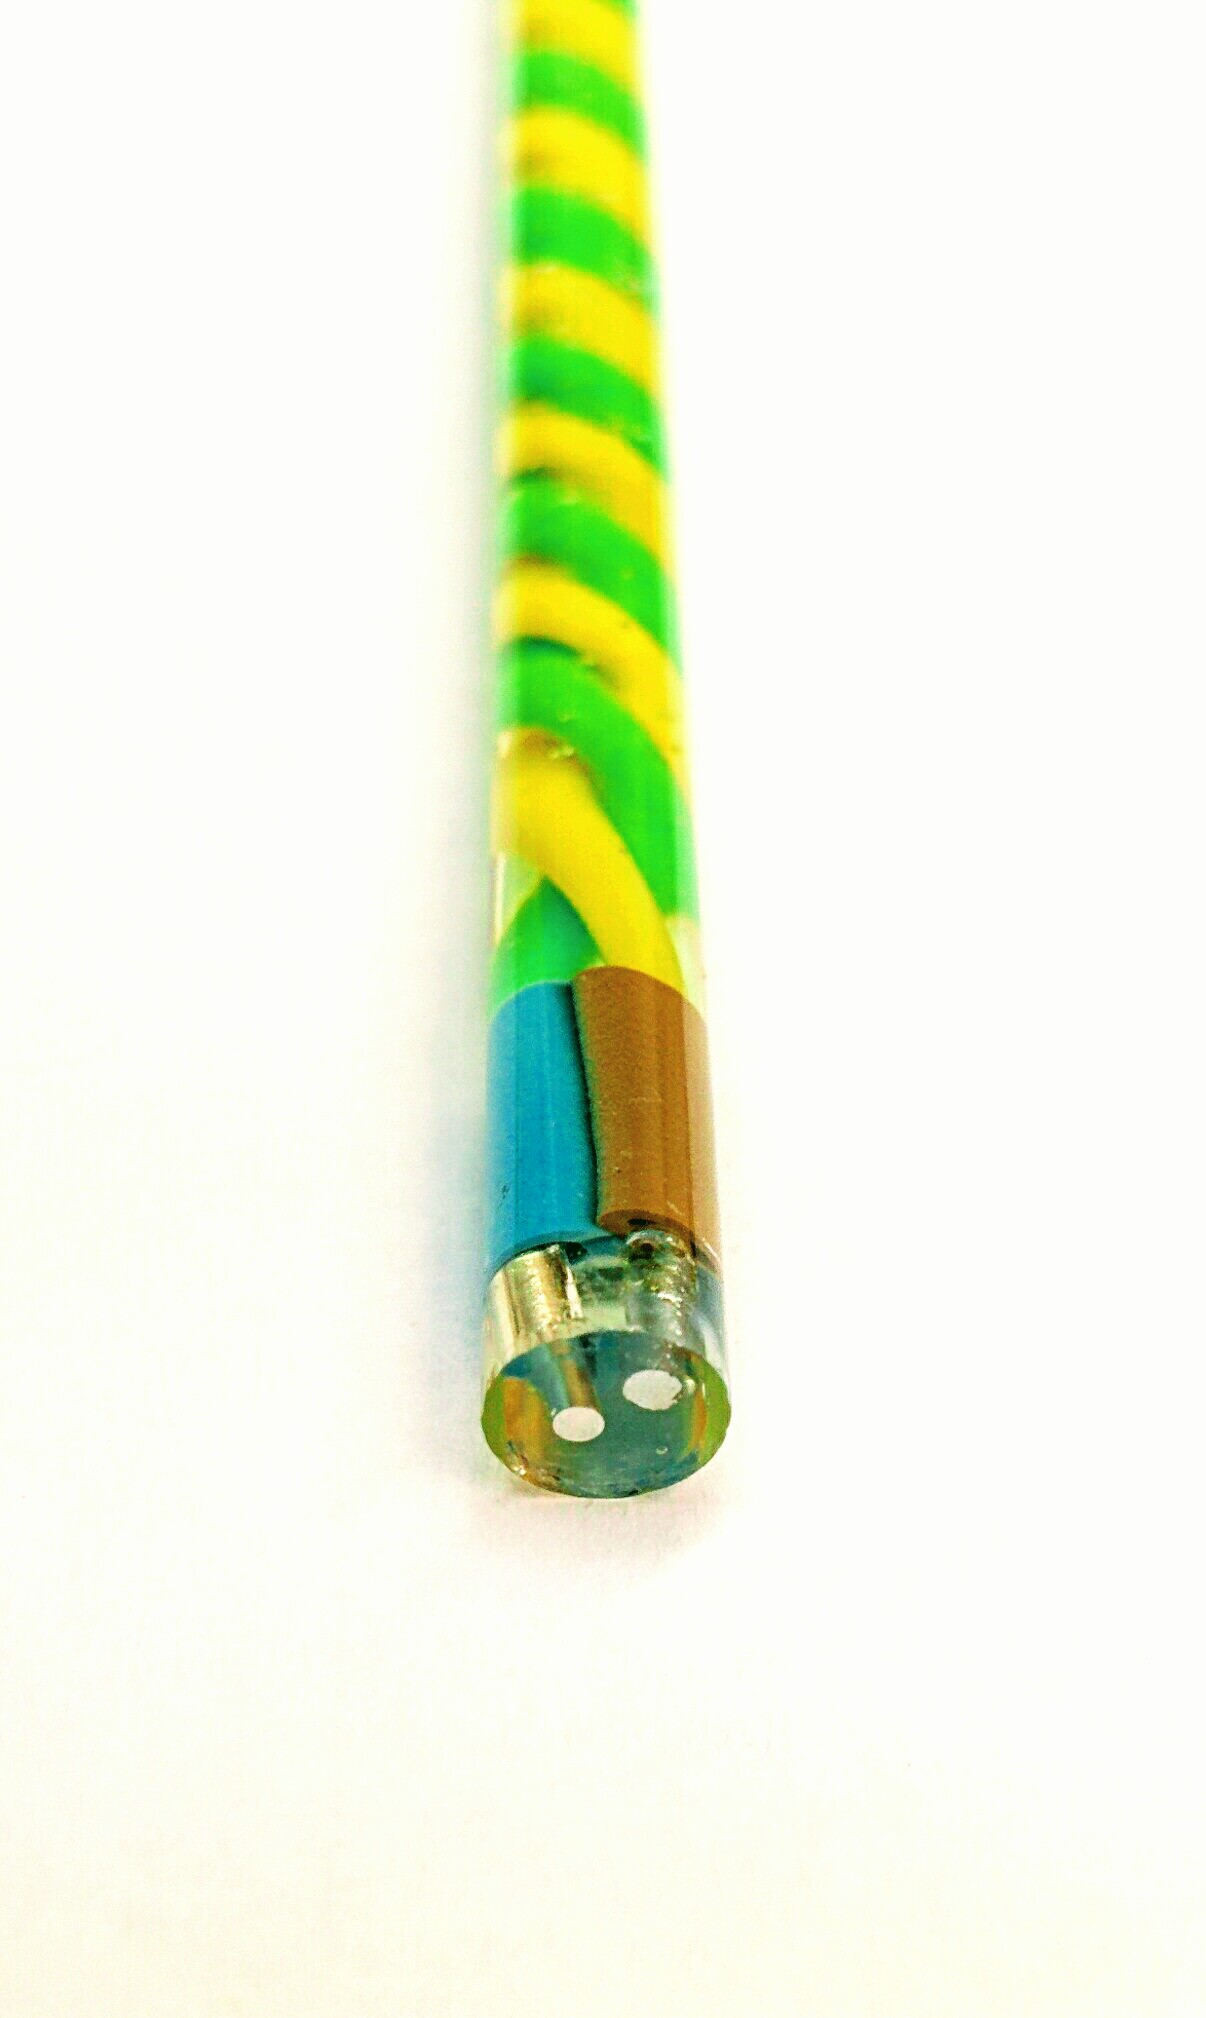
\includegraphics[width=0.165\textwidth]{img/sb_ag_front.jpg}
\caption[Home-made antimony/silver pH-sensitive combined macroelectrodes.]{Home-made antimony/silver pH-sensitive combined macroelectodes.
Left side: top view of two examples, right side: front view, displaying the antimony and silver electrodes. This type of electrode was used to investigate the effect of buffer stirring on response time.}
\label{fig:sb_macro}
\end{figure}

\paragraph{Tungsten pH-sensitive microelectrode}
Since tungsten has the highest melting point of all the elements (3422 $\celsius$), the method described in the previous paragraph cannot be used.
Instead, tungsten microwire with a diameter of $30~\upmu$m (Element-explorer, Montreal, Canada) were sealed into a borosilicate glass capillary ($d_i=1.12~$mm, $d_o=2~$mm, no filament, World Precision Inc., Sarasota, Florida, USA).
To seal the microwire, one end of the capillary was closed with flame.
Then, a 1$~$cm long tungsten microwire was inserted from the other end, and pushed down to the sealed end.
The sealed end was melted again while vacuum was being applied from the open end.
The capillary was kept in the flame until $4-5~$mm, about half of the microwire was sealed into the glass.
To make electrical contact between the microwire and the measuring instruments, a small piece of solder was inserted into the capillary.
The solder was melted in flame, and pushed down to the sealed end of the capillary by a sudden shake of the wrist.
While the solder was still melted, a copper wire was insterted into the solder.
After the solder had cooled down, the electrodes were ready to be used.
Microelectrodes with $30~\upmu$m tungsten filaments from a 100$~$W Tungsram incandescent lightbulb were also prepared, using the same method.
Fig. \ref{fig:tungsten_electrode} shows the tip of the finished tungsten microelectrodes.

\begin{figure}
\centering
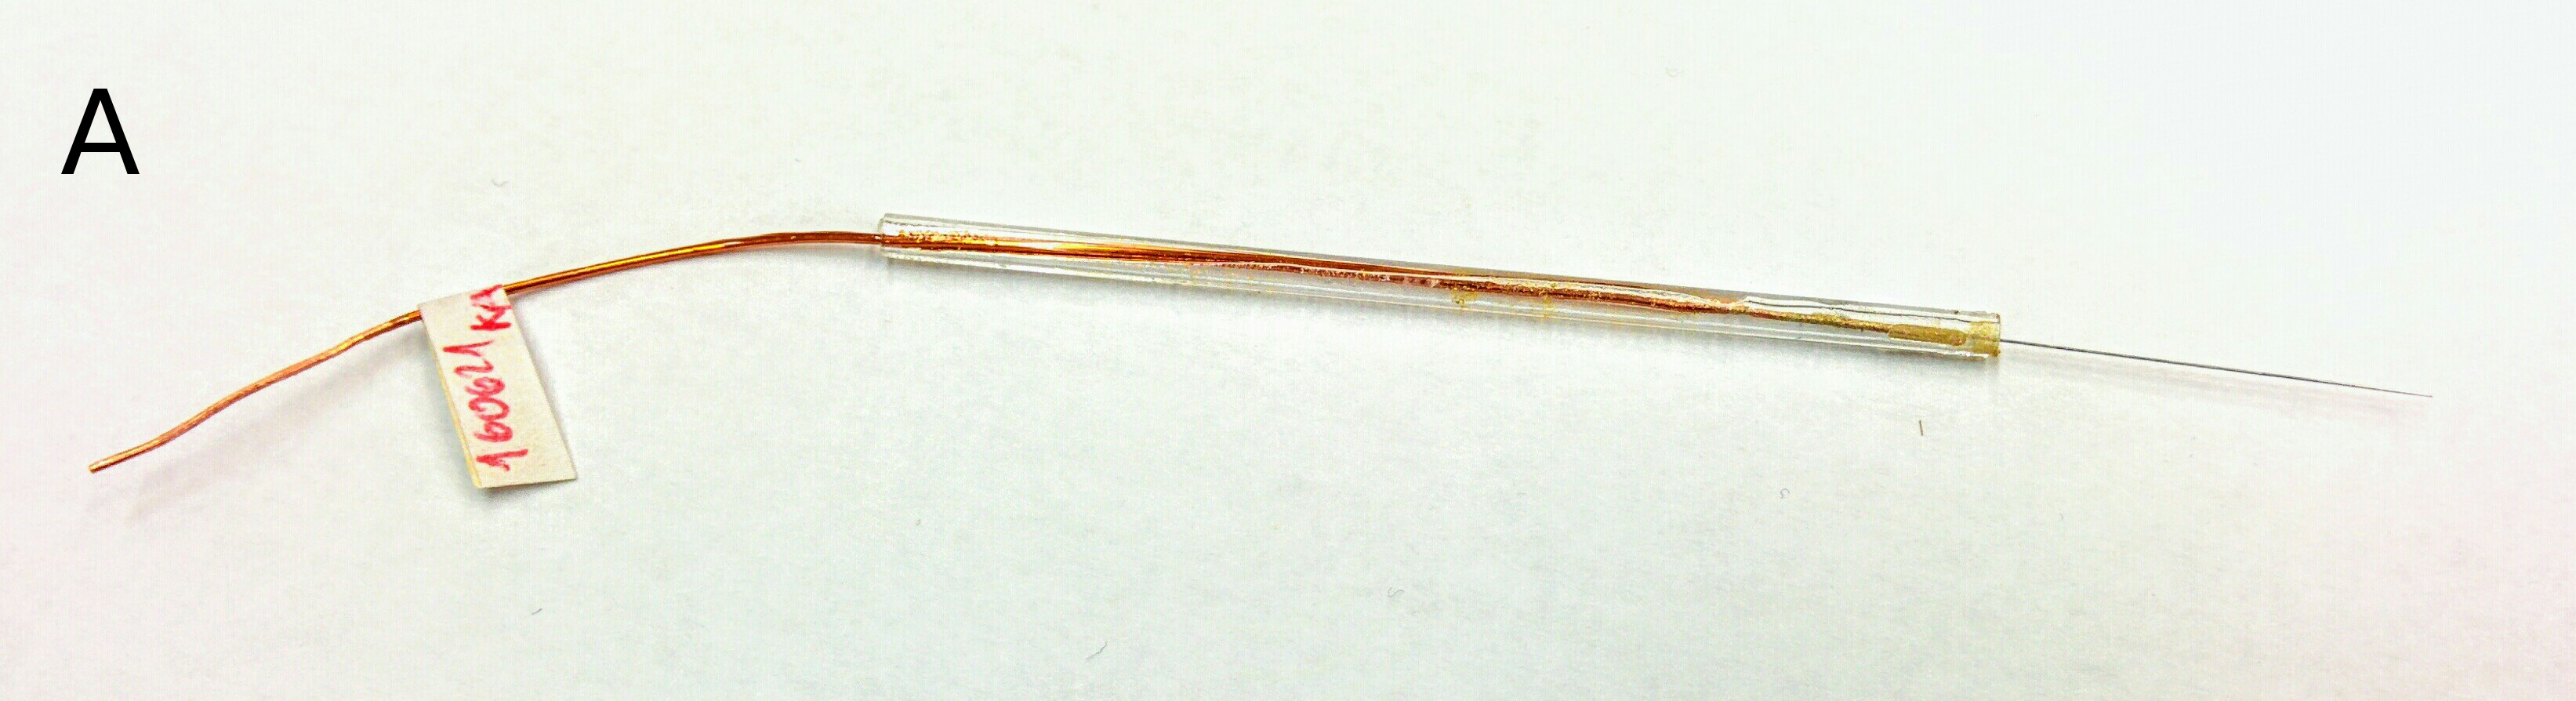
\includegraphics[width=0.9\textwidth]{img/sb_top.jpg}
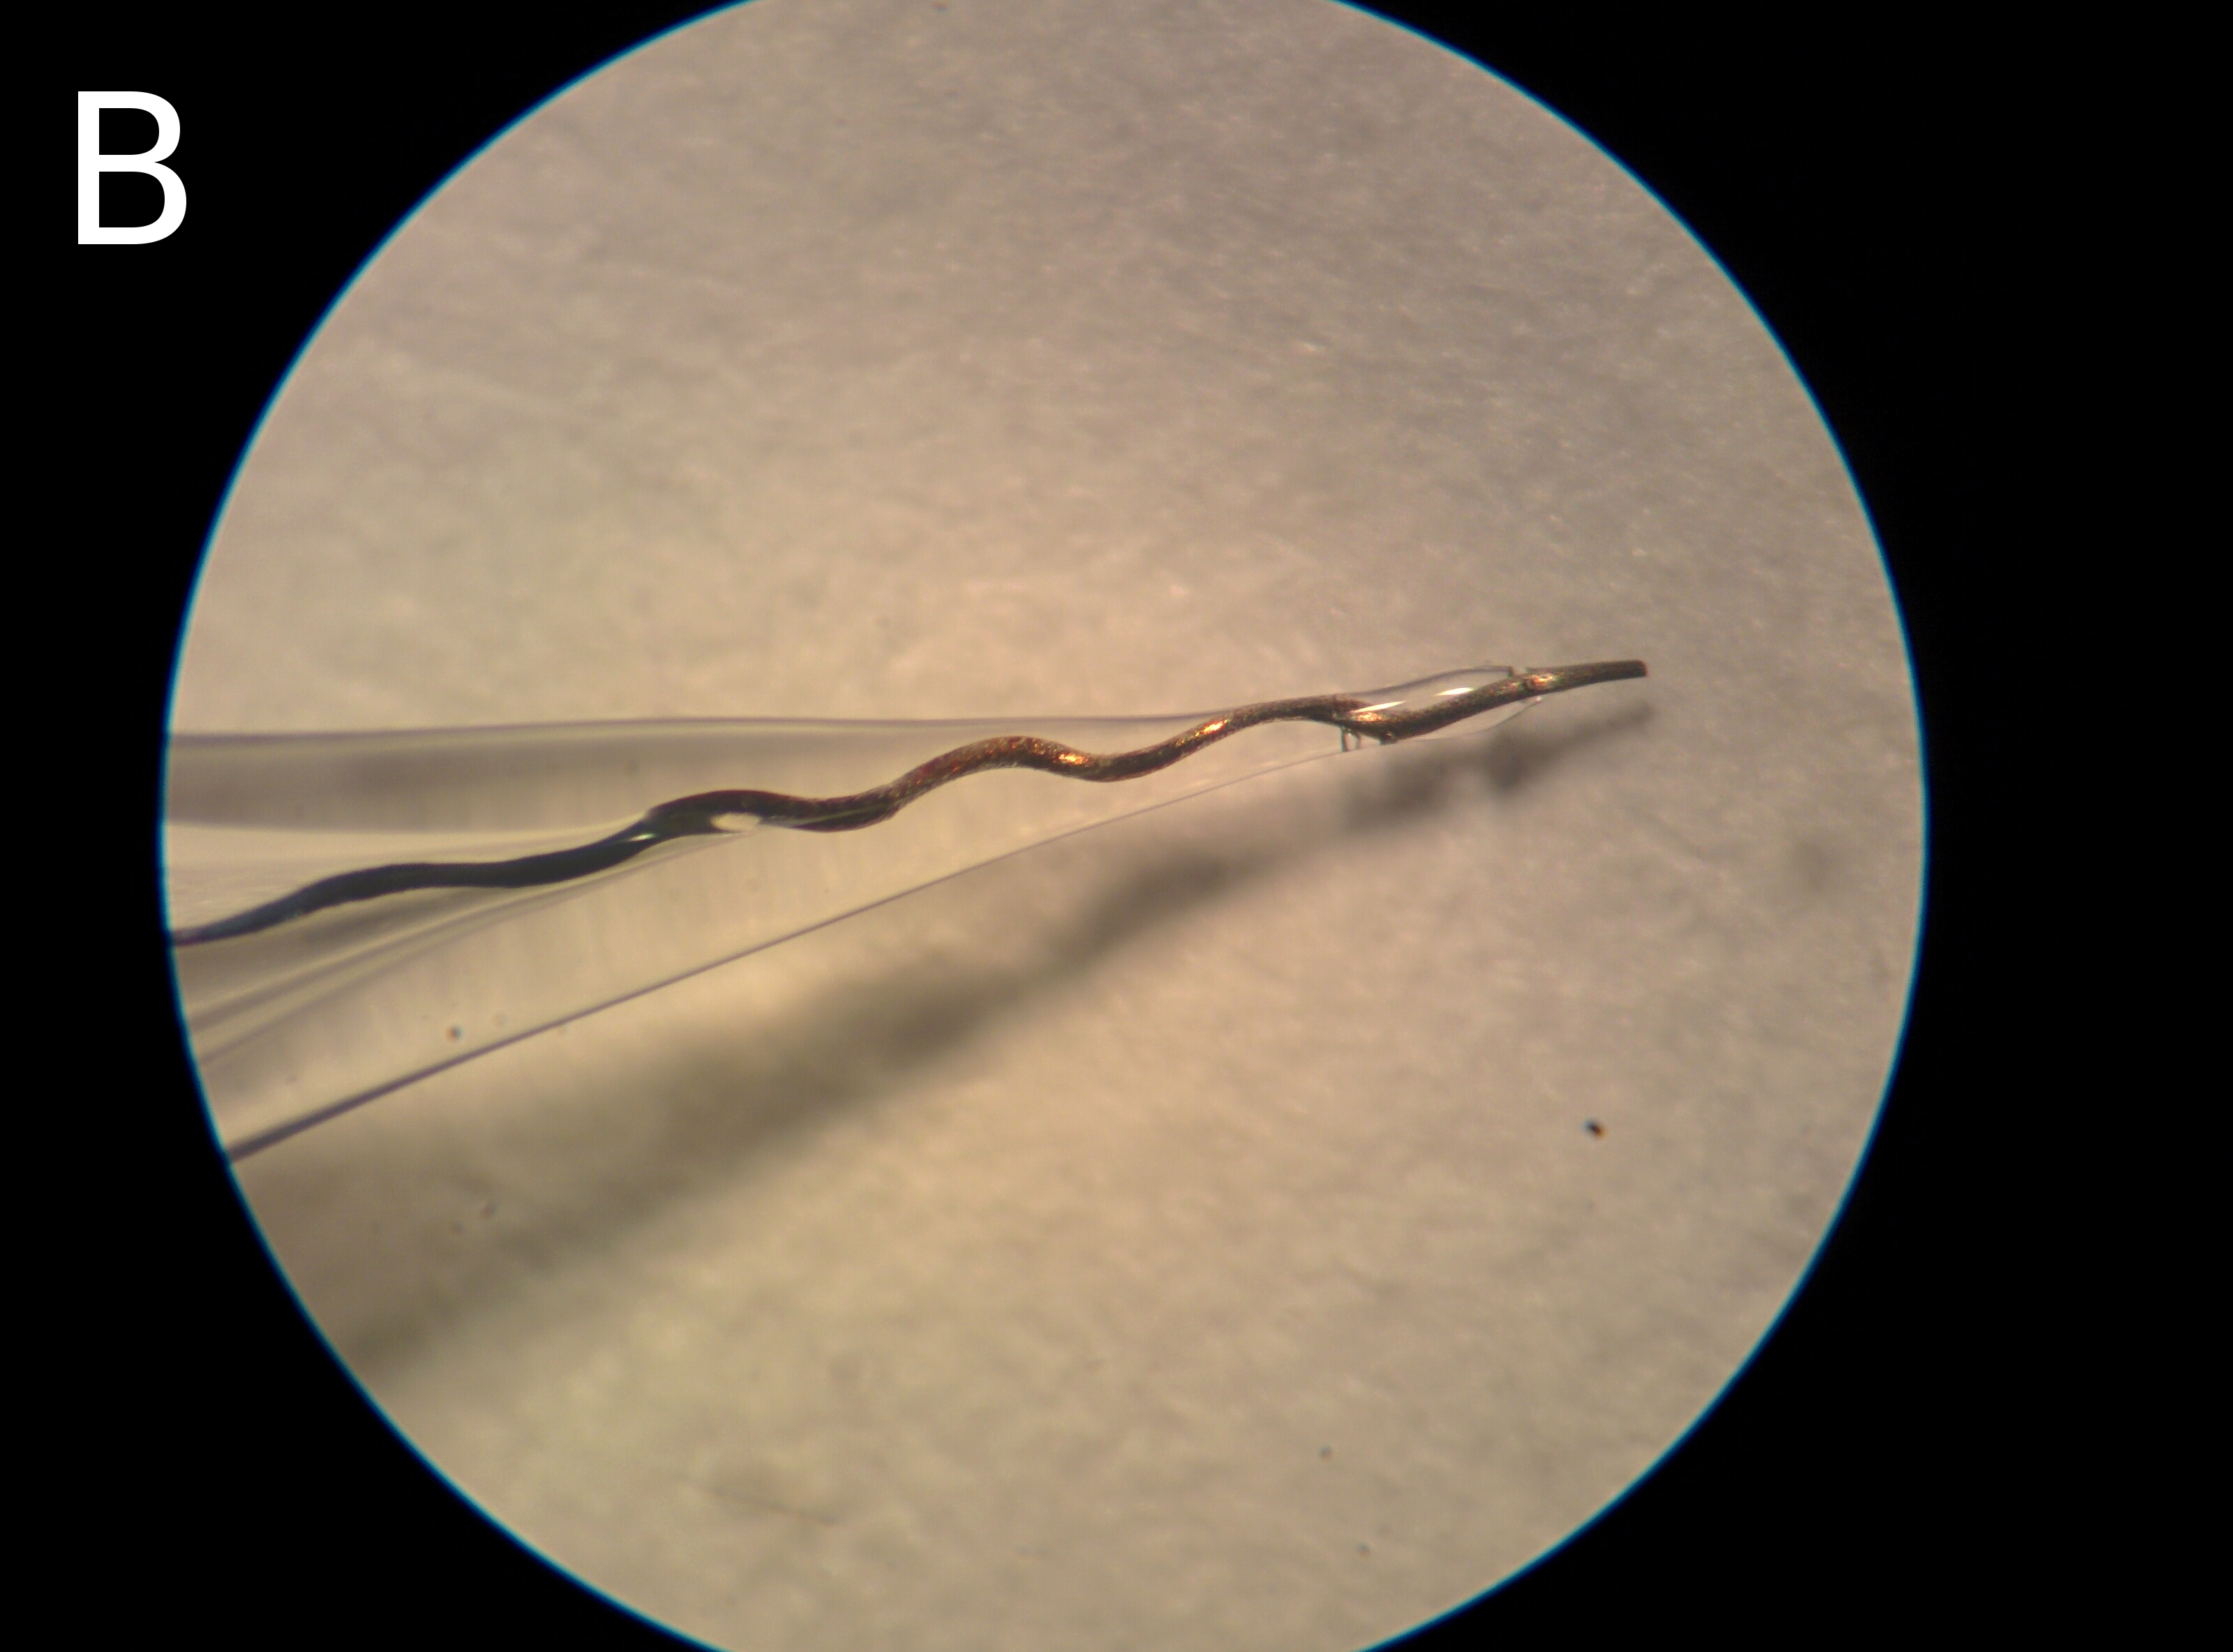
\includegraphics[width=0.45\textwidth]{img/wolfram_electrode1.jpg}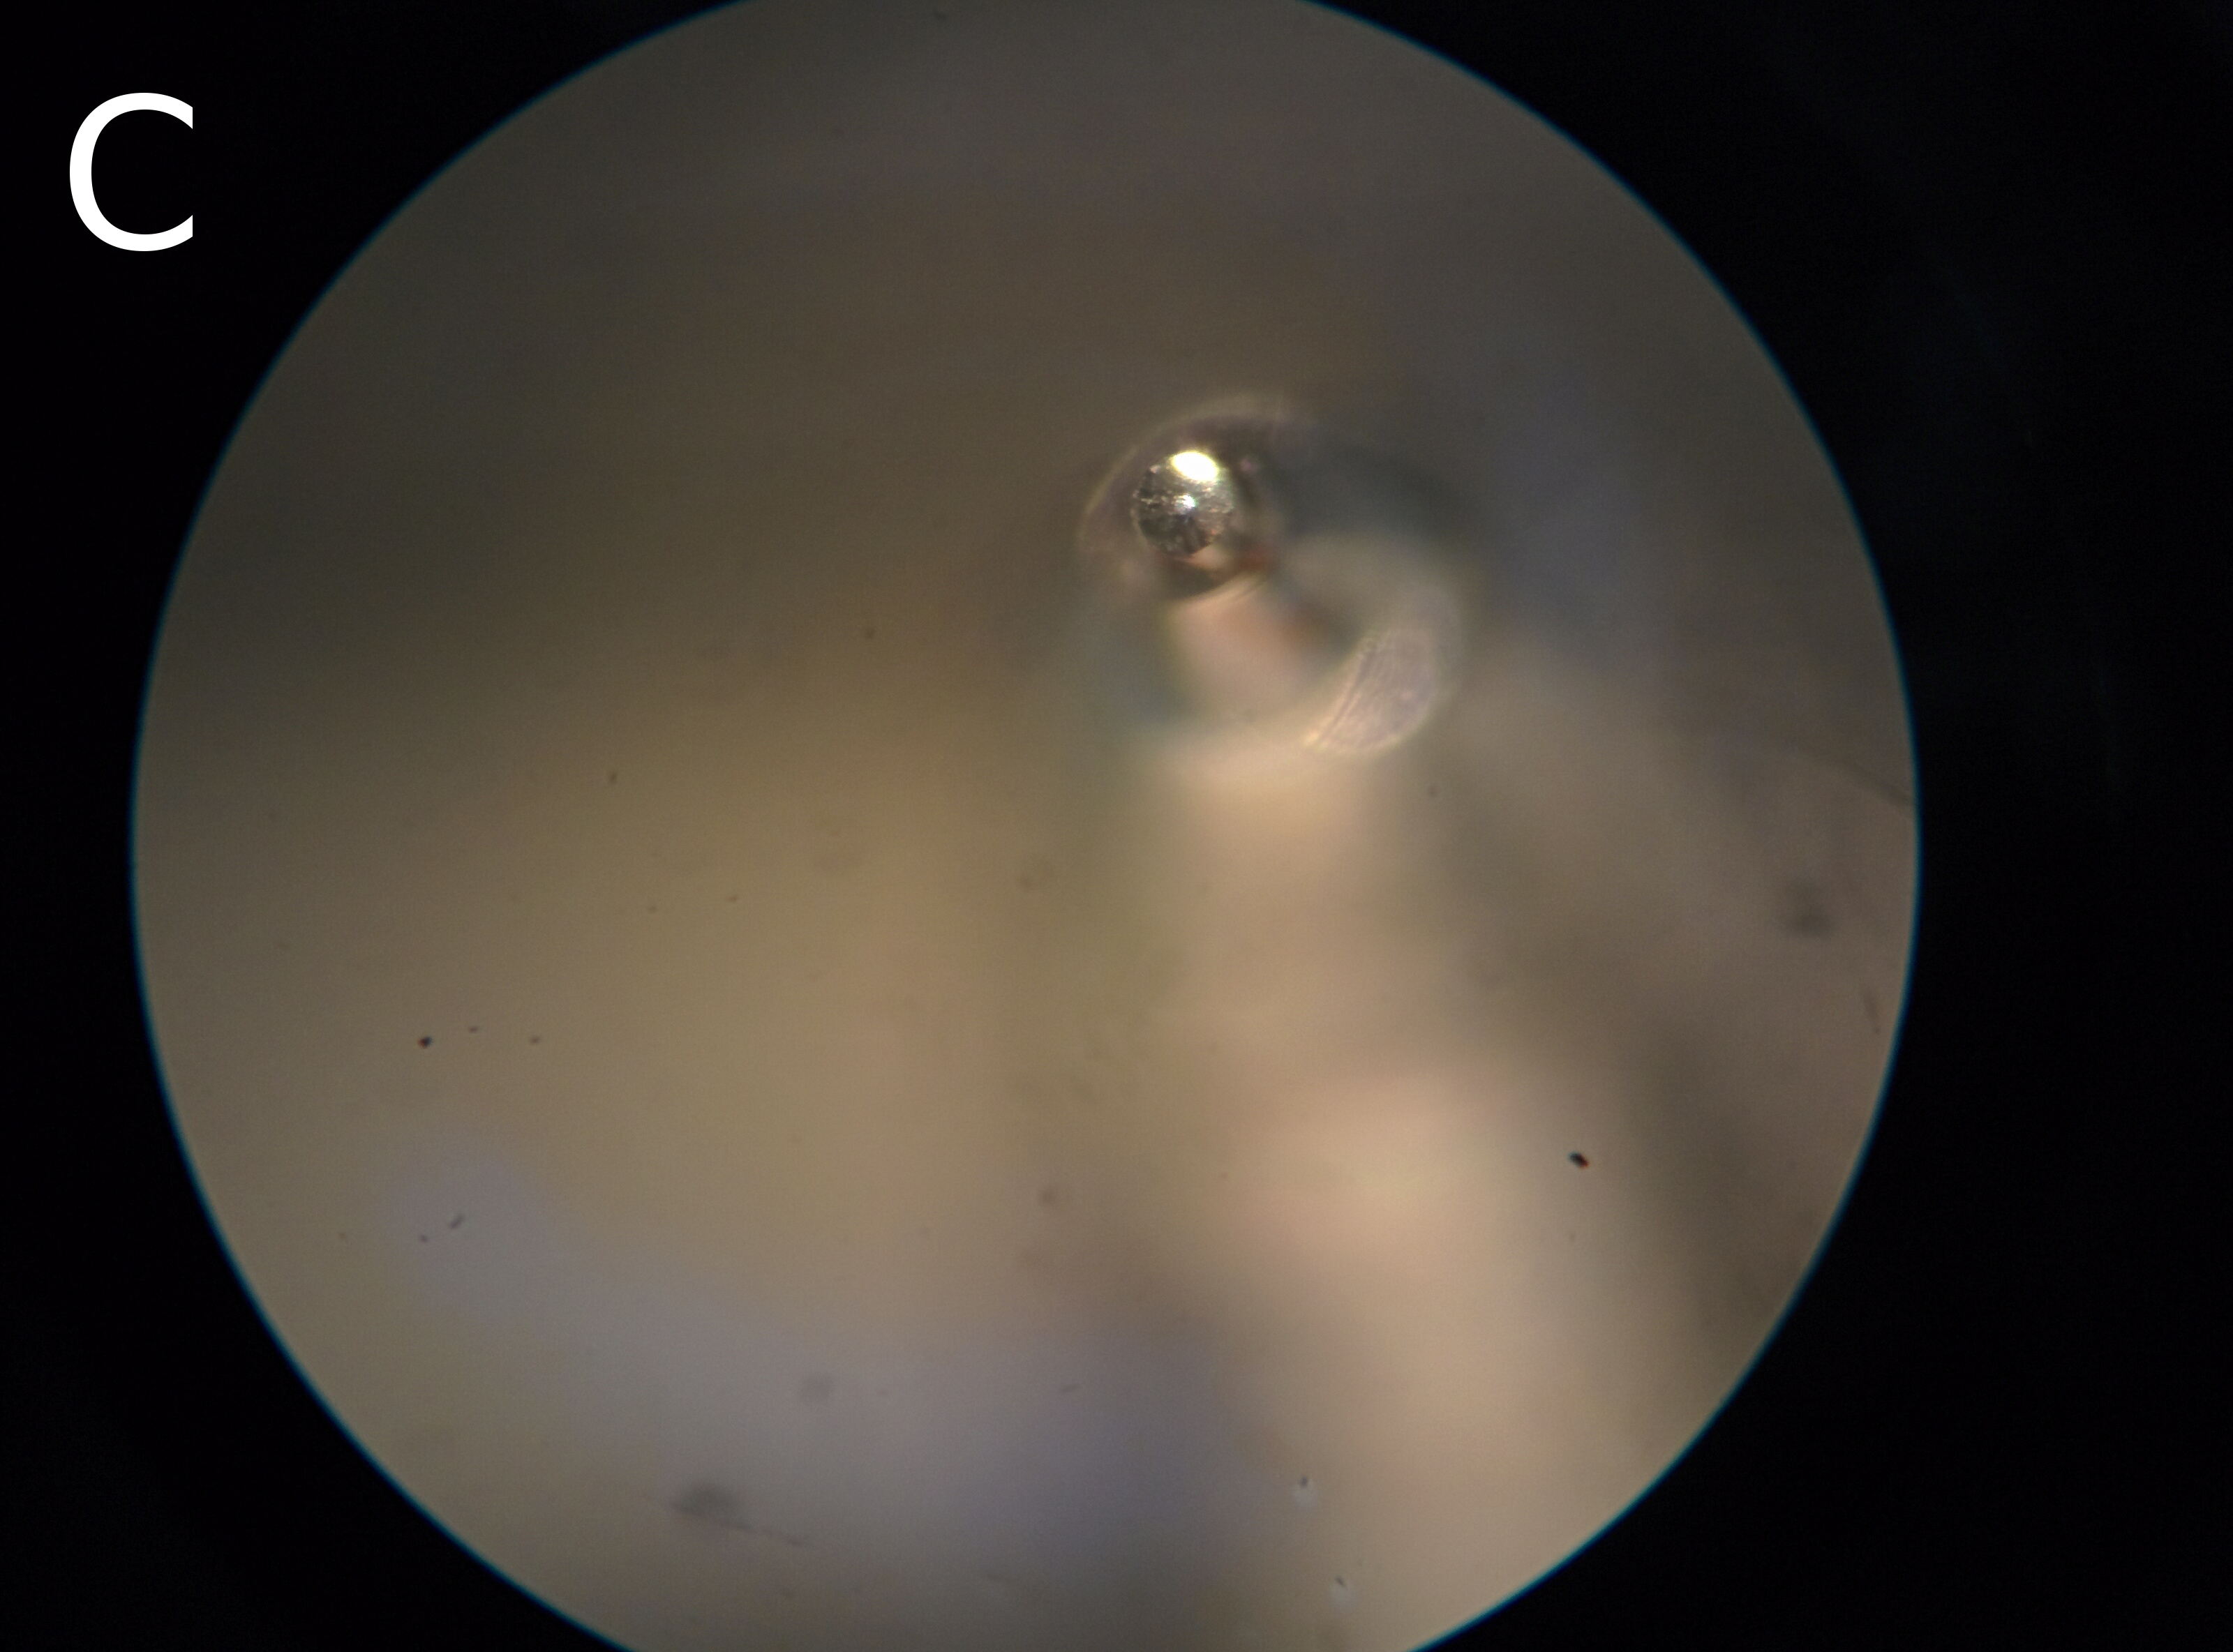
\includegraphics[width=0.45\textwidth]{img/wolfram_electrode2.jpg}

\caption[Antimony and tungsten microelectrodes for local pH measurements.]{(A) Antimony and (B, C) tungsten microelectrodes for local pH measurements.
(B) Side view of the microelectrode prepared from a 100 W Tungsram filament.
(C) Front view of the same electrode.}
\label{fig:tungsten_electrode}
\end{figure}
